Compared to stream processing systems, DDMSes can maintain substantially more state, necessitating the use of more intelligent storage techniques.  However, compared to traditional DBMSes, DDMSes have more information to use when constructing a task-specific storage solution.  

These storage solutions consist of two primary components: First, we can construct datastructures designed specifically for the DDMS' target query workload.  Second, by analyzing the patterns with which operations on the DDMS access data in the database, we can identify a data allocation strategy that reduces IO overhead.

\subsection{Datastructures}
Regardless of whether data is stored in memory, on disk, or across an entire cluster, efficient disk access begins with good representation.  We first consider one instance of a datastructure designed to efficiently support a DDMS' access patterns.  Data in the database can be categorized based on whether it is used in a selection predicate, or purely as data.  For example, consider the query:\texttt{\\
SELECT w.owner, SUM(i.count * p.price)\\
FROM Warehouse w, Inventory i, Product p\\
WHERE w.key = i.warehouse AND p.key = i.product\\
GROUP BY w.owner\\
}
The columns \texttt{owner}, \texttt{count}, and \texttt{price} are an example of the latter, while the two \texttt{key} columns, as well as their foreign key counterparts are examples of the former.  

This categorization into key and data columns, respectively, can make very effective use of a multi-dimensional hash-table.  For example, an intermediate view generated by the DBToaster compiler might contain the join of the Warehouse and Inventory tables.  Rather than storing the view as a series of rows, we can store \texttt{w.owner} and \texttt{SUM(i.count)} in a hash table indexed by \texttt{w.key} and \texttt{i.product}.  

Note that the ability to lookup by partial keys is critical.  Updates to the Product table (like changing the price of a handwoven basket) will read from the example view using only \texttt{p.key} (\texttt{i.product}) and iterating over all matching keys.  This suggests that a series of nested hash-tables would be sufficient, but there is not always a total ordering over the keys.  For example, updates to the Warehouse owner (i.e., the warehouse changes owners) must iterate over all values in the view matching \texttt{w.key}.  

For this purpose, the nested hash-table must be supplemented with (or even replaced by) a series of secondary indices.  Because the query workload is known in advance, the exact set of secondary indices required can be computed at compile time.  An example of this datastructure is shown in Figure \ref{fig:diag:nestedHash}

\begin{figure}
\begin{center}
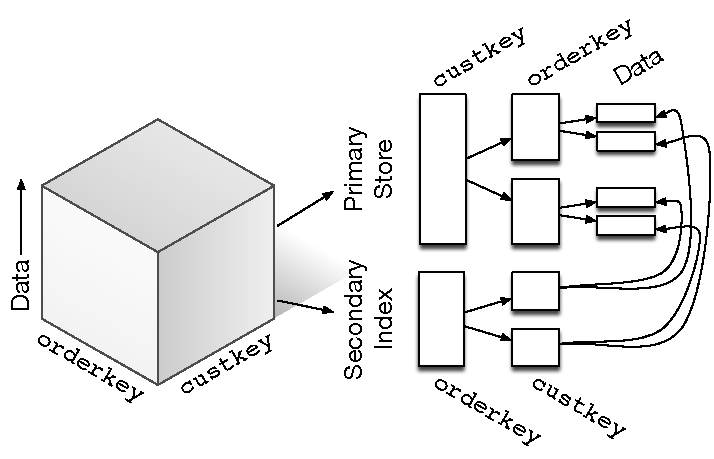
\includegraphics[width=2.5in]{graphics/MultikeyMap}
\end{center}
\caption{Expressing a multi-key iterable hash-table as a nested hash-table with secondary indices.  Secondary indices are optional, and only maintained for access patterns used by one of the DDMS' queries.}
\label{fig:diag:nestedHash}
\end{figure}

%%%%%% should we make any comments here about the relationship between the presence of secondary indices and partitioning schemes?  Otherwise, I'm not sure we have anything to say about maps and datastructures other than (like tables) they're very amenable to horizontal partitioning.

\subsection{Dataflow and Partitioning}
Even with good datastructures, haphazard data placement leads to poor performance.  Though precise workload data may not be available at compile time, a DDMS can still optimize the way it lays out its database across memory, a disk, or even a server cluster, based on the query workload it is constructed with.  An elegant abstraction for doing this is the \textit{dataflow graph}.

Each transition function can be represented as a bipartite directed hypergraph; nodes on the left represent portions of the database being read from, nodes on the right represent a portions being written to, and each hyperedge represents an independent subtask of the transition function.

For example, consider the transition function that results from modifying a Product record in the previous example.  One specific subtask of this transition is a read on the joint Warehouse and Inventory view, and a subsequent write to the output view.  Treating each view as a node, This task has one edge with one read node and one write node.  

We consider database layout in terms of how we distribute, or partition it across a physical medium like memory, disk pages, or a cluster.  Relating this notion to the dataflow graph, a partitioning is an assignment of all nodes in the graph to one (or more, in the case of replication) partition.  

Subdivision of individual views is represented in the dataflow graph as the duplication of  of graph nodes.  Of particular interest, is how the new nodes interact with the hyperedges connected to the original node.  As the split occurs, a node may stay connected to the hyperedge, the hyperedge may likewise be split, or in some cases, only one node will remain connected (eg., the example subtask if the joint view is cut in half based on \texttt{i.product}).  Because the limited set of effects a split can have on each subtask of the dataflow graph, we can exploit this knowledge to choose an effective partitioning scheme.

We could, for instance, partition the joint Warehouse, Inventory view into 4 components by horizontally splitting \texttt{w.key} and \texttt{i.product} each in half.  However, every subsequent update to Products must read from each of the two partitions with a matching \texttt{i.product}, and every insertion to Warehouses must update each of the the two partitions with a matching \texttt{w.key}.  

Conversely, if we split the view into four partitions based on the \texttt{i.product}, updates to Product could be done by accessing a single partition, but updates to Warehouse must now read from four partitions.  Thus, we can choose for an evenly distributed workload, to partition evenly across both keys.

The information used to make these decisions can also come from data-dependent knowledge.  For example, if we can establish a foreign-key dependency between \texttt{i.warehouse} and \texttt{w.key}, we can maintain four partitions along a single axis, while reducing the number of partitions accessed by either subtask to one.

This idea extends to multiple tables.  All nodes not connected to an edge in the dataflow graph are irrelevant for the computation.  Thus, minimizing the number of partitions required to compute by any given transition minimizes the IO overhead of a process.  This is analogous to co-clustering in traditional DBMSes.

%%%%%%%%%%%%%%%%%%%%%%%%%%%%%%%%%%%%%%%%
%In keeping with the DDMS' update-centric view of the world, we view each transition function as a series of write operations, each of which may require one or more read operations.  Both read and write operations may operate on a single row, or iterate over all rows in the table matching a selection predicate.  We can construct a directed hypergraph out of the write operations, with each node representing a table, each out-edge representing a read, and each in-edge representing a write.  We refer to this hypergraph as the transition function's data-flow graph.
%
%This data-flow graph provides a useful mechanism for analyzing the storage, processing, and IO requirements of a query.  In particular it simplifies the analysis of schemes that partition data across multiple physical units, be they disk blocks, disks, or storage servers.  
%
%Regardless of the partitioning scheme selected, each table partitioning will introduce new nodes and edges into the data-flow graph.  Based on the query involved, we can accurately predict how many and which new edges will be introduced.  From this point, we can allocate graph nodes to each partition; 
%
%
%From this point, the partitioning problem begins to resemble a weighted set-cover problem; .  Separating 
%Consider a horizontal partitioning scheme.  Table partitions introduce new nodes and edges into the dataflow graph; we can 
%
%As we partition each table into multiple components, we introduce new nodes and edges into the dataflow graph.  
%
%For example, consider a simple database transition function that emulates the following query\texttt{\\
%INSERT INTO T(a,c')\\
%SELECT a, SUM(c)\\
%FROM R(a,b), S(b, c)\\
%WHERE R.b = S.b\\
%GROUP BY a\\
%}
%
%  partitioning the state of the database 
%This transition function consists of a single hyperedge with two inputs and one output.  The input tables are already narrow, so when, we consider only horizontal partitioning.  We can use the dataflow graph to 
%
%If it becomes necessary to partition the state of the database across multiple disk blocks, disks, or storage servers, we can use the , we could store the entire 
%
%reads from two tables and writes to a third.  This transition function's dataflow graph has a single directed hyperedge with two inputs and one output.  The first reader reads a single 
%
%\begin{itemize}
%\item Overview of read, write, and message costs
%
%\item Partitioning across multiple axis, expanding the dataflow graph into a messaging graph.  
%
%\item Messaging and computational (memory) resources, separability of subgraphs.
%
%\item Basic instantiation - 1 disk or cluster
%
%\item Extensions to the multi-disk case
%\end{itemize}